%//==============================--@--==============================//%
\subsection[3.1 Visão Geral]{\hspace*{0.075 em}\raisebox{0.2 em}{$\pmb{\drsh}$} Visão Geral}
\label{subsec:overview}

\begin{quote}
    ``Recall that the transport layer lies just above the network layer in the protocol stack. Whereas a\textbf{ transport-layer protocol provides logical communication between processes}  running on different hosts, a \textbf{network layer protocol provides logical communication between hosts}.''\cite{Kurose2017}
\end{quote}

\begin{figure}[H]
    \centering
    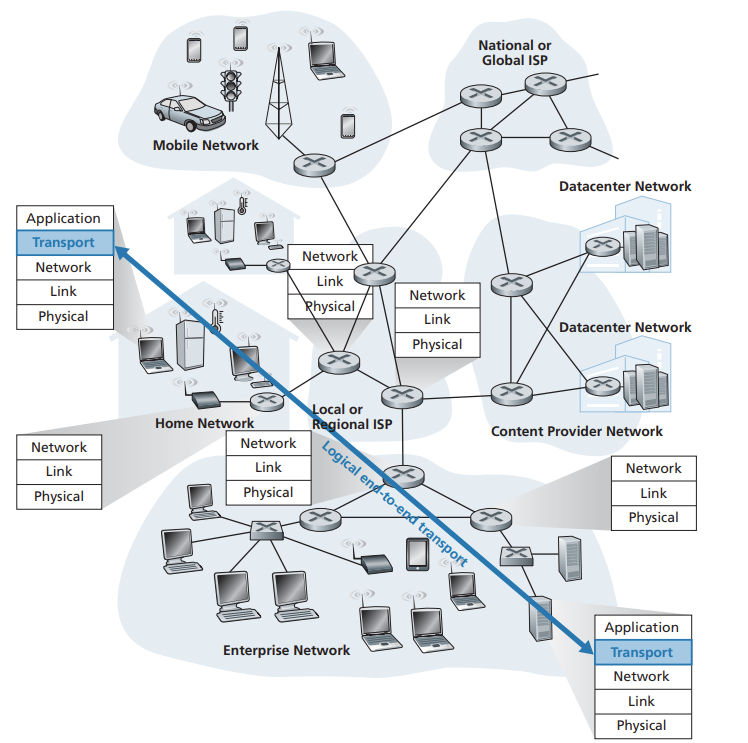
\includegraphics[width = 0.7\linewidth]{img/3/logical-transport.png}
    \caption{``Logical communication between processes''\protect\cite{Kurose2017}}
    \label{fig:logical-transport}
\end{figure}

\noindent A camada de transporte fornece uma abstração sobre a comunicação entre aplicações (processos) que atuam em \textit{hosts} diferentes---``It allows for communication between processes running on different hosts as if they were directly connected, even if they are physically located on opposite sides of the planet''\cite{Kurose2017}. A camada de rede garante o fluxo de \textit{packets} de um \textit{host} a outro, iterando sobre um número arbitrário de redes.

\vspace{0.5 em}
\noindent ``Recall that the Internet makes two distinct transport-layer protocols available to the application layer. One of these protocols is \textbf{UDP} (User Datagram Protocol) and \textbf{TCP} (Transmission Control Protocol)":

\begin{itemize}
    \item \textbf{Entrega fiável e ordenada para unicast: TCP}
    \vspace{-0.25em}    
    \begin{itemize}
        \item Controlo de erros
        \item Controlo de fluxo
        \item Controlo de congestão
    \end{itemize}
    
    \item \textbf{Entrega não-fiável para unicast ou multicast: UDP}
    \vspace{-0.25em}
    \begin{itemize}
        \item Deteção de erros
    \end{itemize}
\end{itemize}

\clearpage
\begin{quote}
    ``Transport-layer protocols are implemented in the end systems but not in network routers. On the sending side, the transport layer converts the application-layer messages it receives from a sending application process into transport-layer packets, known as transport-layer \textbf{segments} in Internet terminology. This is done by (possibly) breaking the application messages into \textbf{smaller chunks} and adding a \textbf{transport-layer header to each chunk} to create the \textbf{transport-layer segment}. The transport layer then passes the segment to the network layer at the sending end system, where the segment is encapsulated within a network-layer packet (a datagram) and sent to the destination.''\cite{Kurose2017}
\end{quote}


%//==============================--@--==============================//%